\chapter{Pendolo di Kater e caduta libera}
\section{Introduzione}

L'obiettivo dell'esperimento è misurare l'accelerazione gravitazionale $g$ attraverso due dei possibili metodi e confrontarli. 


Cronometro digitale con fotocellula a precisione $\pm 0.1 \cdot 10^{-3}\ s$ 

\section{Pendolo di Kater}

\subsection{Strumenti}
Il pendolo di Kater è un pendolo fisico che può essere messo in oscillazione da due punti  $c_1,c_2$ non coincidenti con il suo baricentro $G$. Il pendolo è costituito da un'asta, due masse $m_a = 1400g, m_b=1000g$ mobili e due coltelli posizionato nei punti $c_1,c_2$ che ne permettono l'oscillazione. 
Il periodo del pendolo dipende dal punto di oscillazione:

$$ T_1 = 2 \pi \sqrt{\frac{L_1}{g}} = 2 \pi \sqrt{\frac{I_1}{m_a gh_1}}$$


$$ T_2 = 2 \pi \sqrt{\frac{L_2}{g}} = 2 \pi \sqrt{\frac{I_2}{m_b gh_2}}$$

dove $L_i$ la lunghezza ridotta del pendolo, $I_i$ il momenti d'inerzia del pendolo appeso per il punto $i-esimo$  e $h_i$, la distanza del punto $i$ dal baricentro. 
\\
Se si individuano i due punti nel quale il periodo $T_1 = T_2$ allora l'equazione si riduce a:

$$ T = \ 2 \pi \sqrt{\frac{D}{g}}$$
\\
La distanza $D= h_1 + h_2 $  è nota e nel nostro caso $ D= 99.4 cm$. Misurando quindi il periodo $T$, possiamo calcolare $g$. 
\subsection{Metodo sperimentale}
\begin{itemize}

\item Si pone in oscillazione il pendolo dal coltello $c_1$ e si misura $T_1$, e si ripete l'operazione per il coltello $c_2$, misurando $T_2$. 
\item Mantenendo fissa la massa $m_a$ ad una distanza $d = 15.4cm$ da $c_1$,  si allonta o si avvicina la massa $m_b$ . Successivamente ripetere il punto precedente. 
\item La procedura viene ripetuta fino a trovare la posizione nel quale $T_1 \simeq T_2$. 
\item A questo punto si costruisce un grafico in cui si riporta il periodo $T_1$ e$ T_2 $ in funzione della distanza $x$ di $m_b$ da un coltello. 
\item Per diminuire l'incertezza nella misura del periodo, abbiamo misurato il tempo totale di 10 oscillazioni. Dividendo il tempo totale per N, numero oscillazioni, si ottiene il periodo medio. 

\end{itemize}

\subsection{Dati}
Nella tabella sono raccolti tutti i periodi $T_1,T_2$ misurati in secondi. \\
\textit{Nota:} $d$ è la distanza tra il coltello $c1$ e la massa $m_b$. 
In grassetto è evidenziato il punto di sospensione del pendolo a cui sono riferiti i periodi scritti di seguiti. 
\begin{center}
\begin{tabular}{*{8}{c}}
$d$& $7.4cm$ & $11.7cm$ & $13.5cm$  & $15cm$ & $17.9cm$ & $84.4cm$ & $81.3cm$ \\
\midrule
 \textbf{Coltello1}&& & & & & \\
&2.1197 &2.0040&2.0279 &1.9809 & 1.9211 & 1.9934 & 1.9735\\
 &2.1125&2.0041 &2.0029&1.9796 & 1.9207 & 1.9932 & 1.9744 \\
 &2.1179&2.0043 &2.0021&1.9816 & 1.9264 & 1.9931 & 1.9746 \\
 &2.1204&2.0062 &2.0042&1.9794 & 1.9253 & 1.9932 & 1.9755 \\
 &2.1189&2.0060 &2.0026&1.9821 & 1.9113 & 1.9932 & 1.9765 \\
 &2.1129&2.0052&2.0012&1.9805 & 1.9278 & 1.9934 & 1.9769 \\
&2.1125 &2.0050&2.0014&1.9802 & 1.9278 & 1.9937 & 1.9770 \\
&2.1131 &2.0061&2.0008&1.9804 & 1.9277 & 1.9941 & 1.9760 \\
 &2.1143&2.0046&2.0036&1.9810 & 1.9278 & 1.9937 & 1.9754 \\
 &2.1131&2.0058&2.0005& 1.9831 & 1.9278 & 1.9935 & 1.9750 \\
\textbf{Coltello2} && & & & & \\
&2.0279&2.0041&1.9983 &1.9934 & 1.9882 & 1.9946 &	1.9802 \\
&2.0284&2.0043&1.9983 &1.9946 & 1.9902 & 1.9939 &	1.9812 \\
&2.0289&2.0062&1.9967 &1.9911 & 1.9907 & 1.9943 &	1.9820 \\
&2.0289&2.0060&1.9978 &1.9919 & 1.9908 & 1.9941 &	1.9818 \\
&2.0288&2.0052&1.9978 &1.9940 & 1.9907 & 1.9940 &	1.9819 \\
&2.0288&2.0050&1.9986 &1.9923 & 1.9907 & 1.9952 &	1.9813 \\
&2.0288&2.0061&1.9986 &1.9939 & 1.9888 & 1.9954 &	1.9816 \\
&2.0288&2.0046&1.9988&1.9934 & 1.9898 & 1.9943 &	1.9818 \\
&2.0286&2.0058&2.0001 &1.9914 & 1.9898 & 1.9947 &	1.9812  \\
&2.0286&2.0040&1.9994 &1.9958 & 1.9878 & 1.9941 &	1.9810 \\
\bottomrule
\end{tabular}
\end{center}

\subsection{Analisi}
Possiamo ora iniziare l'analisi dei dati. Innanzitutto, calcoliamo il valore medio $T$ e l'incertezza associata alla distanza $d_i$.
\begin{center}
\begin{tabular}{c   c}
\begin{tabular}{c|c|c}
$d$ & $T_1(s)$ & $\sigma_{t_1}$ \\
\midrule
7.4 & 2.1158 & 0.001\\
11.7 & 2.0085 & 0.006\\
13.5 & 2.0021 & 0.00039\\
15.0 &  1.9806 & \\
17.9 & 1.9244 &\\
21.0 & 1.9076 &\\
81.3 & 1.9755&\\
84.4 & 1.9935&\\
\end{tabular}
&
\begin{tabular}{c|c|c}
$d$ & $T_2(s)$ & $\sigma_{t_2}$ \\
\midrule
6.9 & 2.02865 & 0.001\\
11.7 & 2.0075 &\\
13.5 & &\\
15.0 &  1.9806 &\\
17.9 & 1.9244 &\\
21.0 & 1.9076 &\\
81.3 & 1.9755&\\
84.4 & 1.9935&\\
\end{tabular}
\end{tabular}
\end{center}


$\pm\sigma$

\section{Caduta libera}


\subsection{Raccolta dati}
Tutti i valori riportati in tabella sono in millisecondi.
\begin{center}
\begin{tabular}{r|*{14}{c}}
\textbf{20 cm} & 197 & 199 & 197 & 200 & 199 & 203 & 200 & 203 & 196 & 199 & 196 & 199 & 197 & 205\\
& 198 & 199 & 198 & 197 & 199 & 198 & 197 & 198 & 200 & 198 & 199 & 199 & 198 & 204\\
\midrule
\textbf{35 cm} & 265 & 265 & 265 & 261 & 262 & 263 & 266 & 262 & 269 & 266 & 261 & 263 & 262 & 261\\
\midrule
\textbf{50 cm} & 314 & 315 & 314 & 321 & 319 & 316 & 315 & 315 & 315 & 314 & 314 & 315\\
\midrule
\textbf{60 cm} & 347 & 345 & 346 & 347 & 344 & 344 & 348 & 345 & 346 & 344 & 345 & 345\\
\midrule
\textbf{90 cm} & 424& 424& 424& 423& 425& 424& 426& 423& 424& 423& 422& 425& 423\\
\end{tabular}
\end{center}

\begin{center}
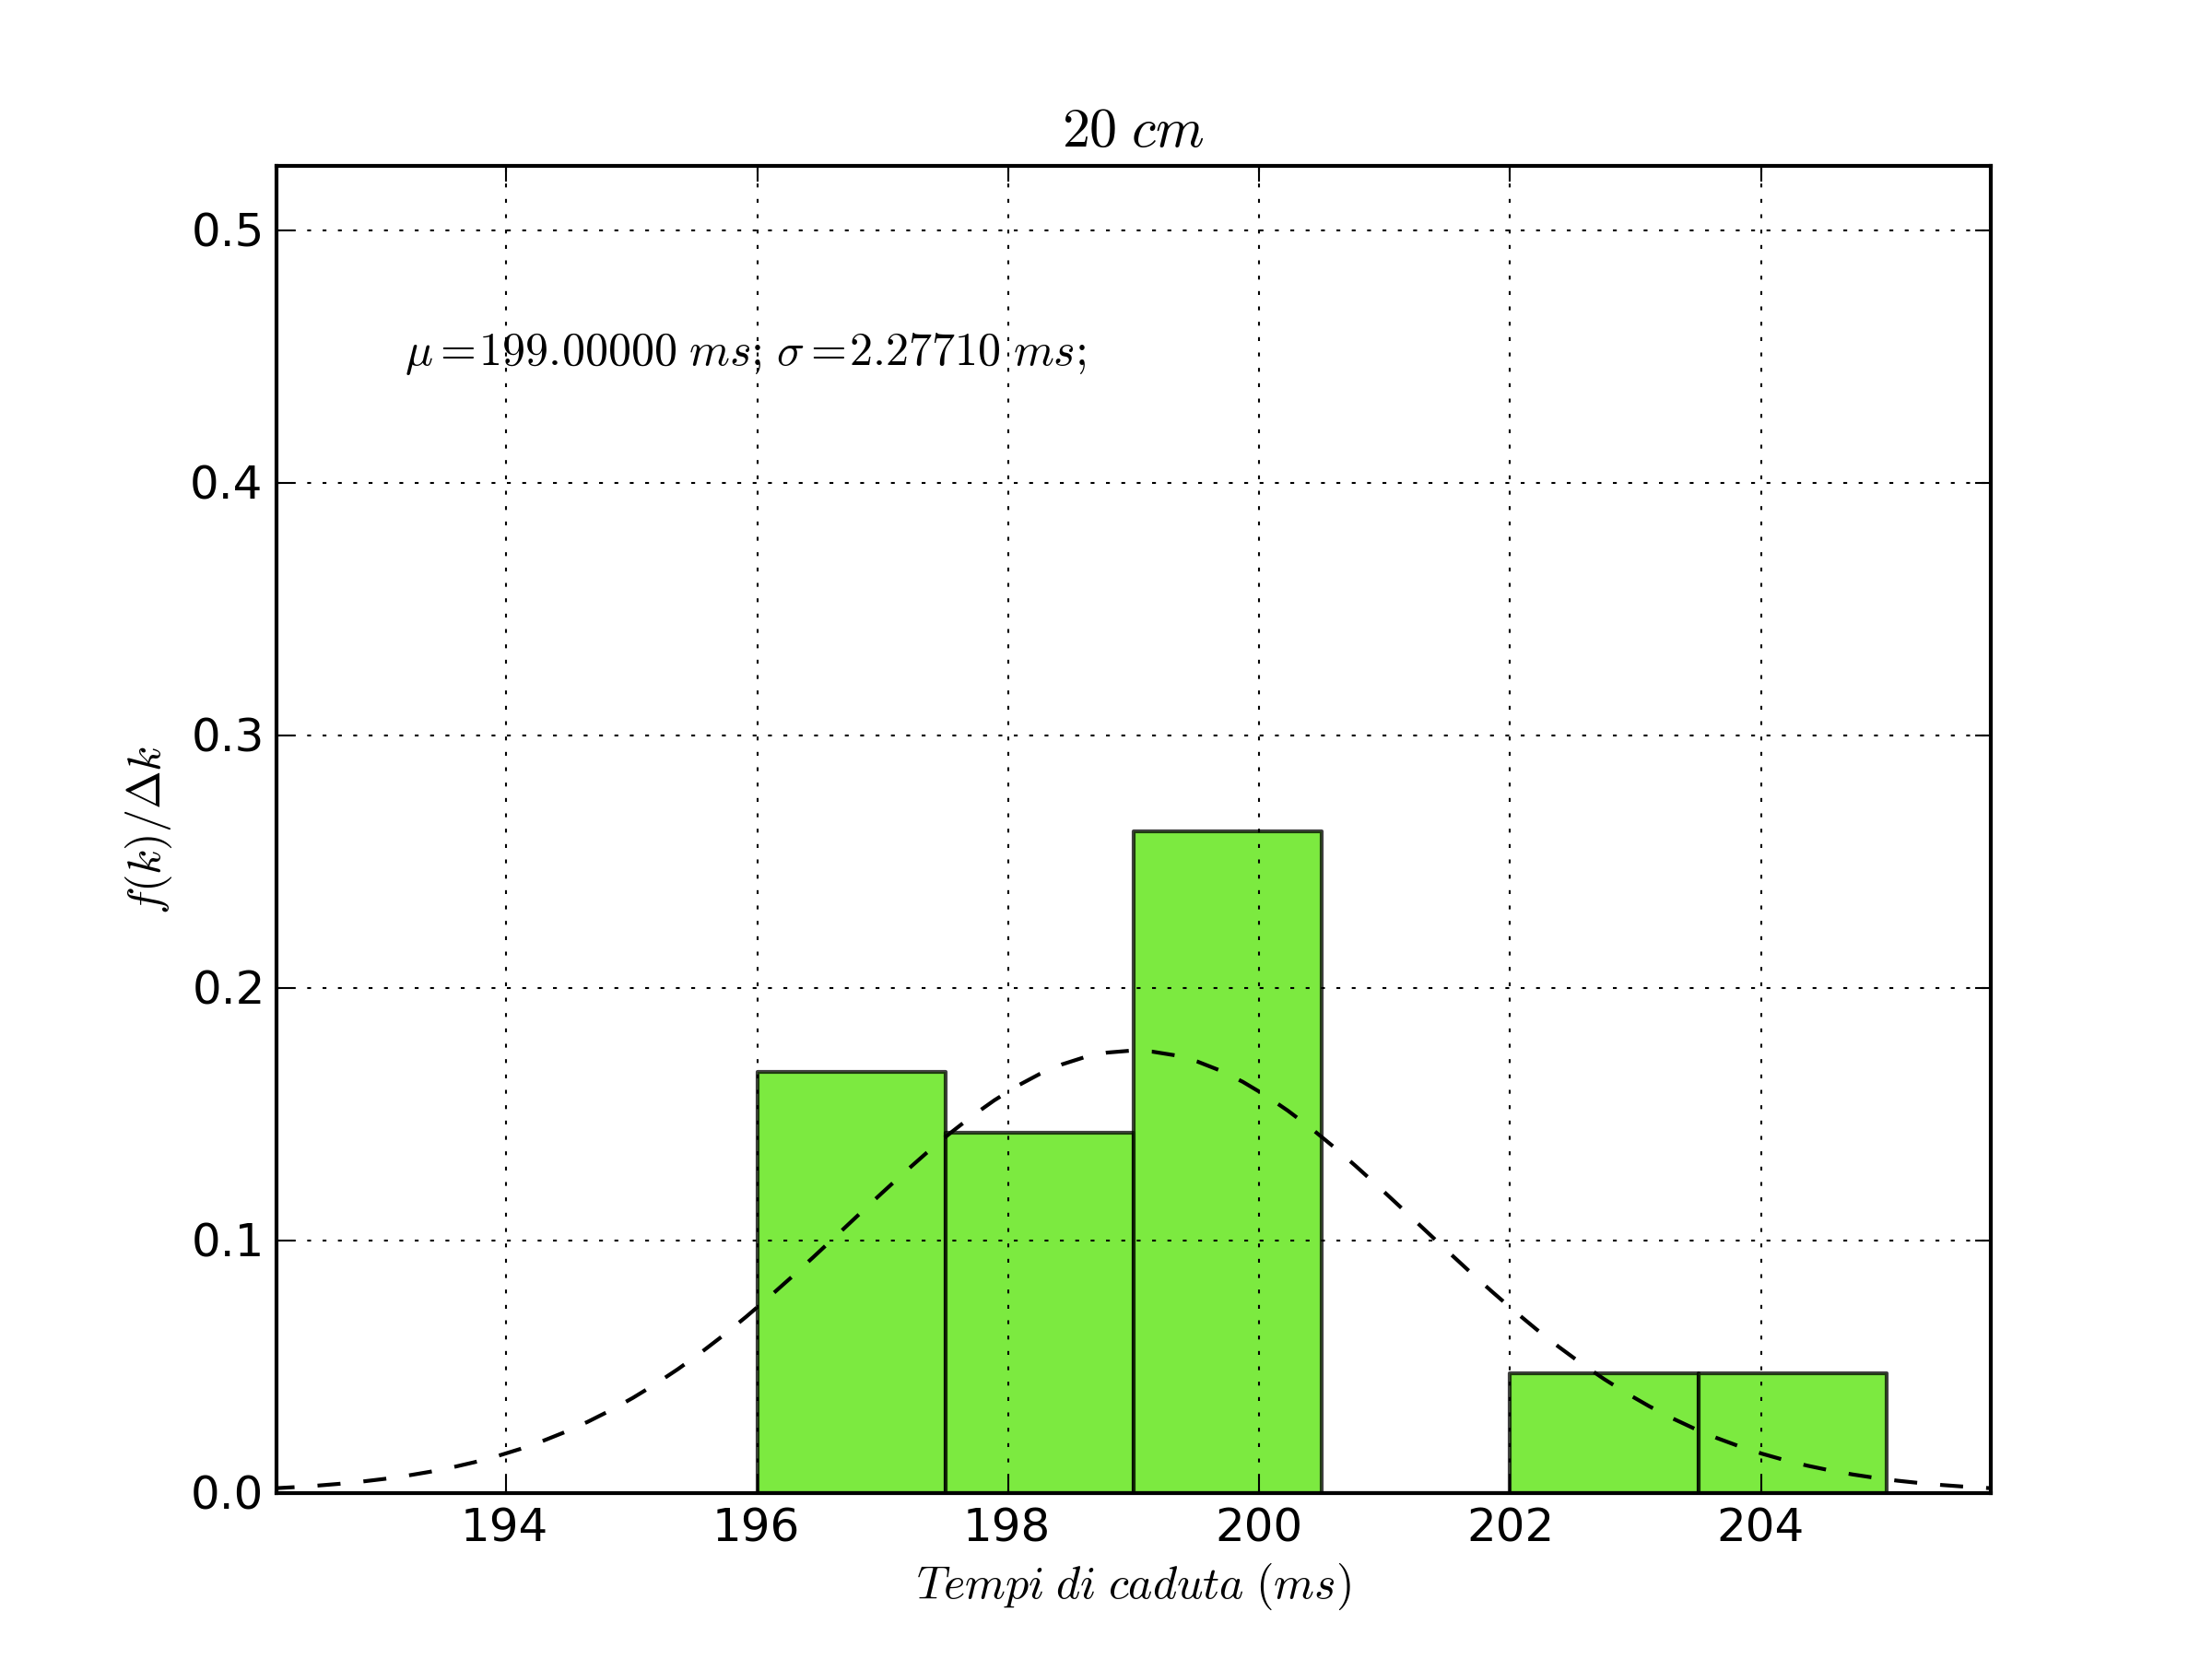
\includegraphics[scale=0.75]{../grafici/20cm.png}
$$\sigma_{\bar{x}} = 0.430\ ms$$
$$\mathrm{Stima\ di\ g} = 10.10\ m/s^2$$
$$\mathrm{Stima\ (corretta)\ di\ g} = 9.80\ m/s^2 $$
$$\frac{\Delta g_c}{g} = 0.00072$$
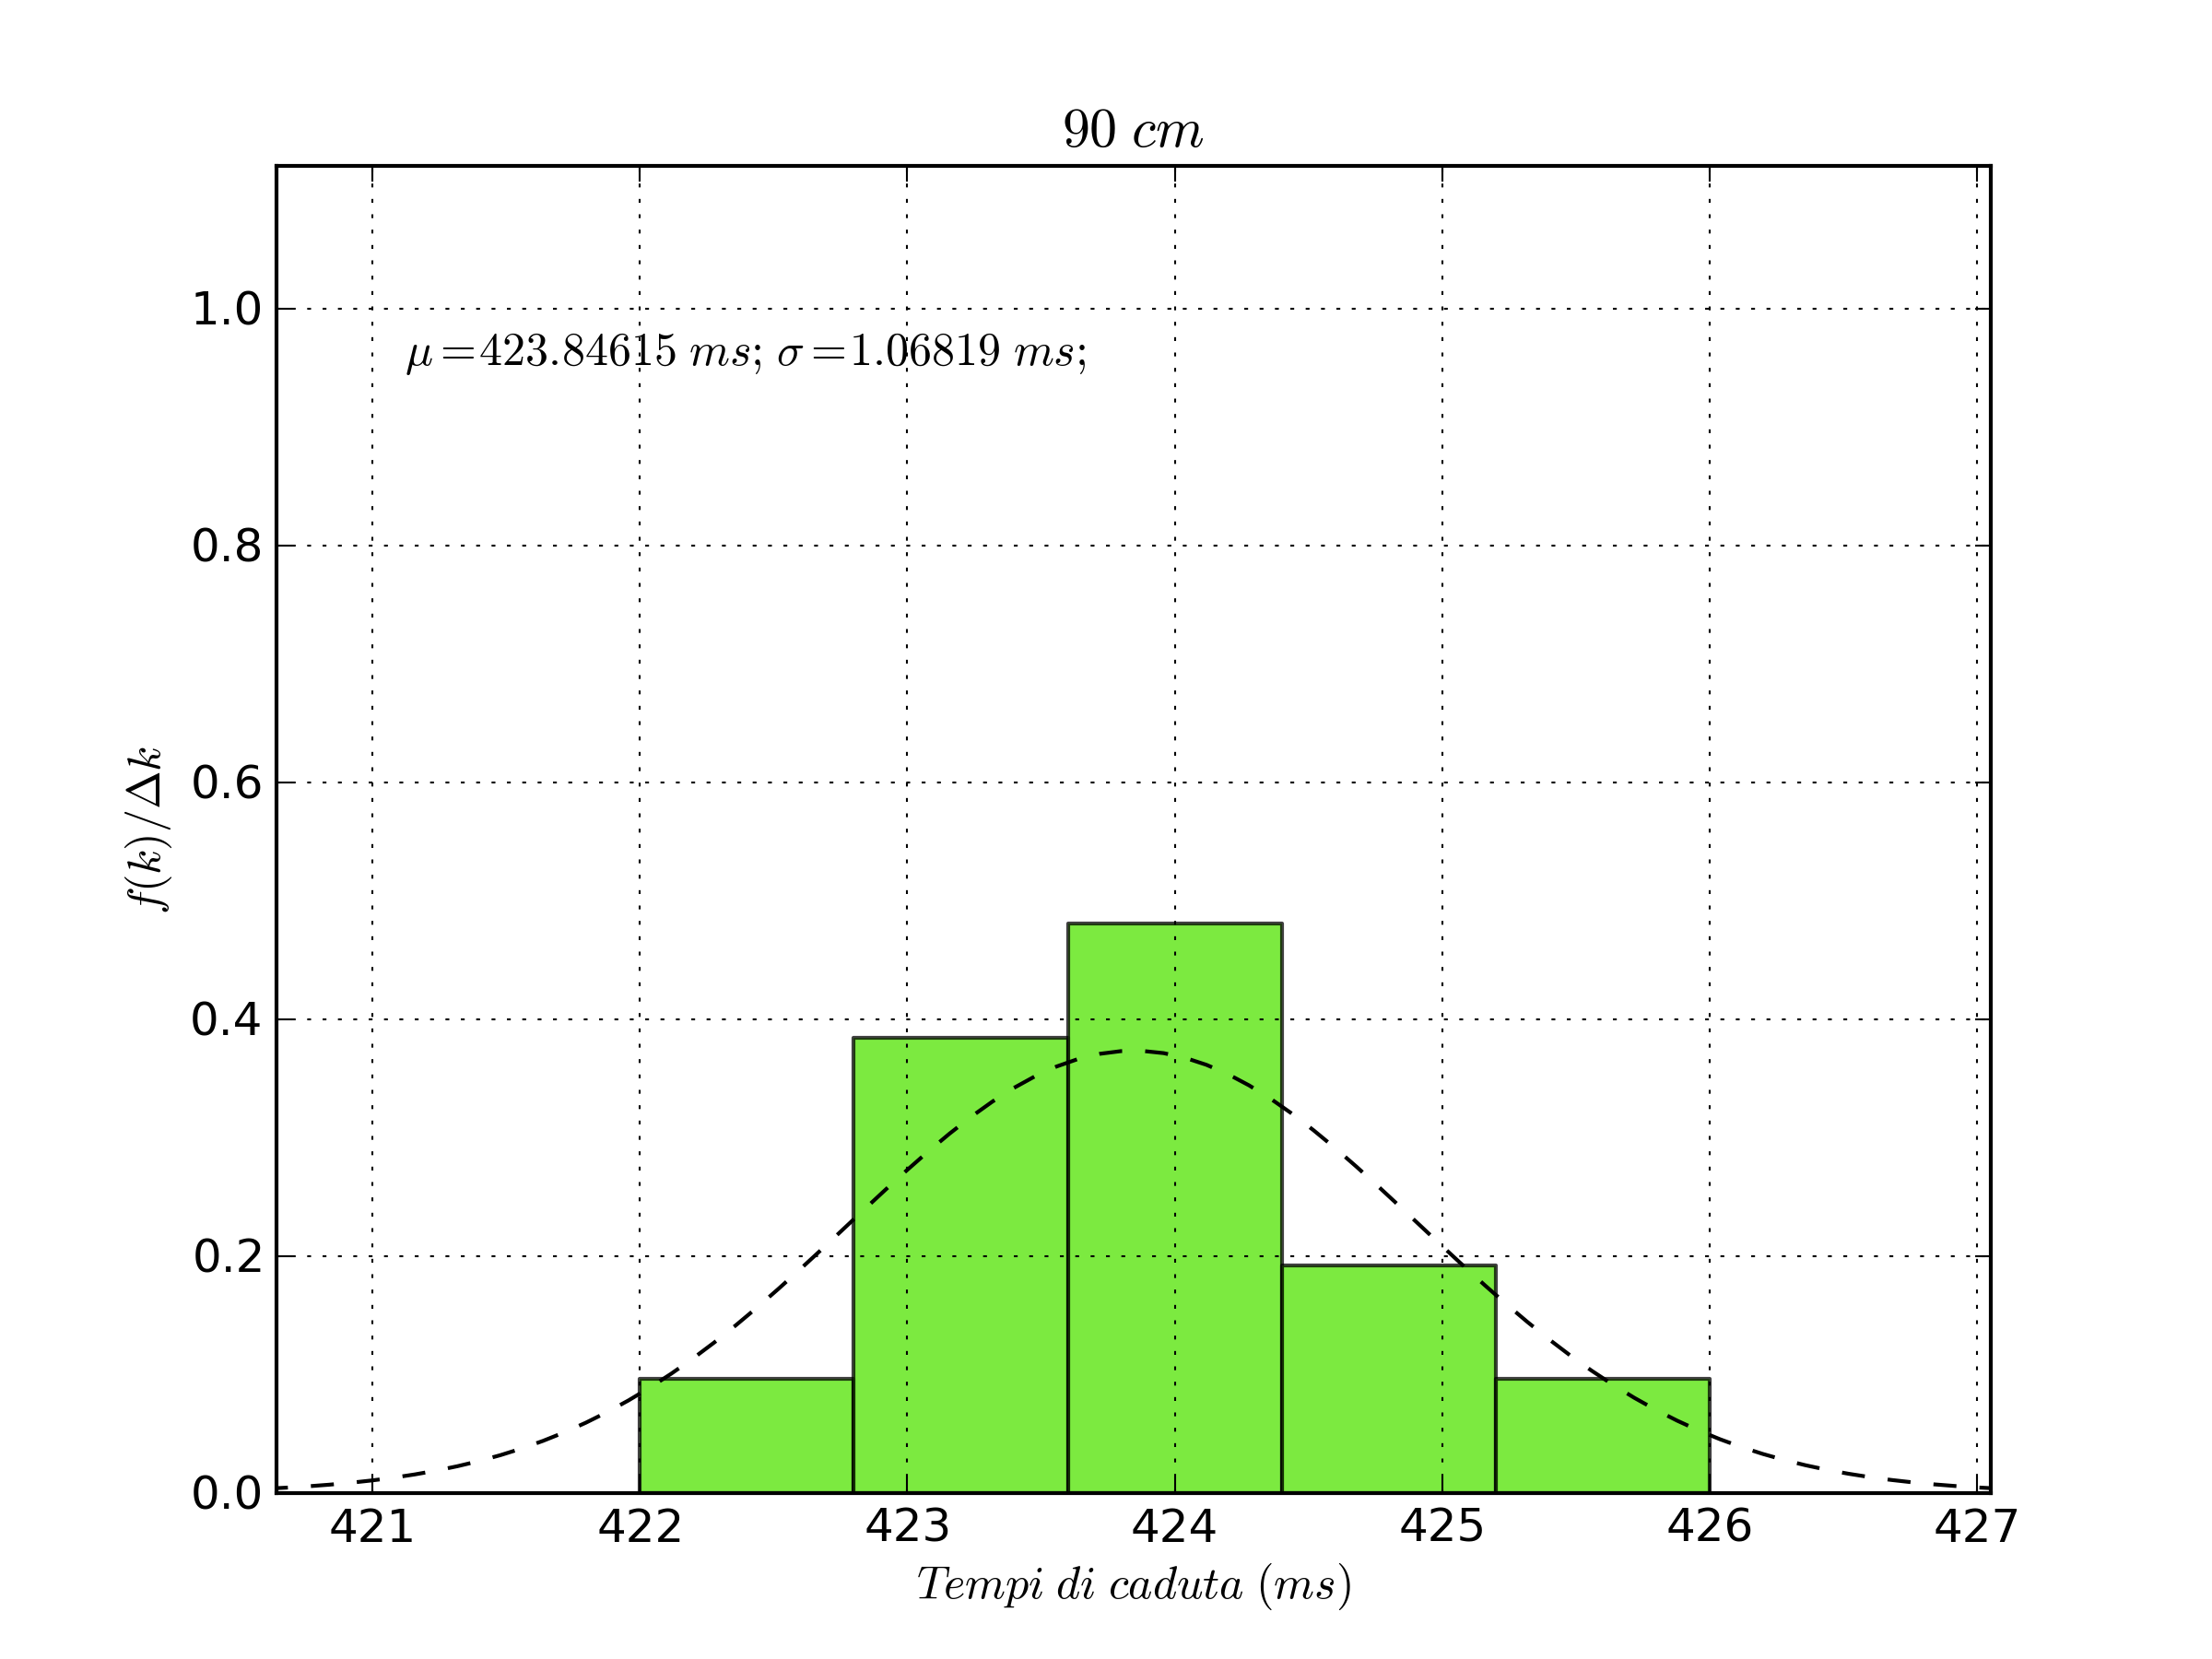
\includegraphics[scale=0.75]{../grafici/90cm.png}
$$\sigma_{\bar{x}} = 0.296\ ms $$
$$\mathrm{Stima\ di\ g} = 10.02\ m/s^2$$
$$\mathrm{Stima\ (corretta)\ di\ g} = 9.88\ m/s^2 $$
$$\frac{\Delta g_c}{g} = 0.00707$$
\end{center}

La correzione applicata è di 3 ms aggiunti al tempo segnato dal cronometro. Non avendo dati più precisi sulla costruzione del cronometro stesso, assumiamo questo tempo come [delay]... scrivi meglio!

\begin{center}
\begin{tabular}{c|c|c|c|c}
$h$ (m) & $g$ (m/s$^2$) & $g_c$ (m/s$^2$) & $\Delta g/g$ & $\Delta g_c/g$\\
\midrule
0.20 & 10.10 & 9.80 & 0.02964 & 0.00072 \\
0.35 & 10.07 & 9.85 & 0.02659 & 0.00362 \\
0.50 & 10.04 & 9.85 & 0.02354 & 0.00435 \\
0.60 & 10.05 & 9.88 & 0.02475 & 0.00718 \\
0.90 & 10.02 & 9.88 & 0.02138 & 0.00707 \\
\end{tabular}
\end{center}


\section{Conclusioni}